\section{Deadlock BPaxos}
In this section, we present \defword{Deadlock BPaxos}, a slight tweak to
Unanimous BPaxos. Like Unanimous BPaxos, Deadlock BPaxos can choose a command
in one round trip, but unlike Unanimous BPaxos, Deadlock BPaxos only requires
fast quorums of size $\SuperQuorumSize$ (the same as Fast Paxos).
%
While Deadlock BPaxos is safe, it is not very live. There are failure-free
situations in which Deadlock Paxos can deadlock. Thus, Deadlock BPaxos, like
Unsafe BPaxos, is a purely pedagogical protocol. In the next section, we fix
Deadlock BPaxos's lack of liveness.

\subsection{Pruned Dependencies}
We discuss Deadlock BPaxos momentarily, but first we pause to understand one of
the key invariants that it maintains. Recall that in order to preserve
\invref{ConflictInvariant}, both Simple BPaxos and Unanimous BPaxos maintain
\invref{SimpleBpaxosInvariant}.
%
Deadlock BPaxos does not maintain this invariant. Instead, it maintains an
invariant that is weaker but still sufficient to imply
\invref{ConflictInvariant}. The motivation for the weaker invariant is as
follows.

Imagine a Deadlock BPaxos node $b_i$ sends command $x$ to the dependency
service in instance $I$, and the dependency service responds with $(I, x,
\deps{I})$. Let $I' \in \deps{I}$ be one of $I$'s dependencies. Assume that
that $b_i$ knows that $I'$ has been chosen with value $(y, \deps{I'})$. Further
assume that $I \in \deps{I'}$. In this case, there is no need for $b_i$ to
include $I'$ in the dependencies of $I$! \invref{ConflictInvariant} asserts
that if two instances $I$ and $I'$ are chosen with conflicting commands $x$ and
$y$, then either $I \in \deps{I'}$ or $I' \in \deps{I}$. Thus, if $I'$ has
already been chosen with a dependency on $I$, then there is no need to propose
$I$ with a dependency on $I'$.
%
Similarly, if $I'$ has been chosen with $\noop$, then there is no need to
propose $I$ with a dependency to $I'$ because $x$ and $\noop$ do not conflict.
%
Let $(I, x, \deps{I})$ be a response from the dependency service. Let $P
\subseteq \deps{I}$ be a set of instances $I'$ such that $I'$ has been chosen
with $\noop$ or $I'$ has been chosen with $I \in \deps{I'}$. We call $\deps{I}
- P$ the \defword{pruned dependencies} of $I$ with respect to $P$. Deadlock
BPaxos maintains \invref{PrunedDependencies}. \invref{DependencyService} and
\invref{PrunedDependencies} imply \invref{ConflictInvariant} (see
\appendixref{DeadlockExample} for proof).

\begin{invariant}\invlabel{PrunedDependencies}
  For every instance $I$, a value $v$ is chosen in instance $I$ only if $v =
  (\noop, \emptyset)$ or if $(I, x, \deps{I})$ is a response from the
  dependency service and $v = (I, x, \deps{I} - P)$ where $\deps{I} - P$ are
  the pruned dependencies of $I$ with respect to some set $P$.
\end{invariant}

\subsection{The Protocol}
Deadlock BPaxos is identical to Unanimous BPaxos except for the
following modifications.
%
First, Deadlock BPaxos fast quorums are of size $\SuperQuorumSize$.
%
Second, every Fast Paxos acceptor maintains a partial BPaxos graph in exactly
the same way as the set of Deadlock BPaxos nodes. When an acceptor learns that
an instance $I$ has been chosen with value $(x, \deps{I})$, it adds $I$ to its
partial BPaxos graph labelled with $x$ and with edges to every instance in
$\deps{I}$. We will see momentarily that whenever a Deadlock BPaxos node $b_i$
sends a phase 2a message to acceptors with value $v = (x, \deps{I} - P)$ for
some pruned dependencies $\deps{I} - P$, $b_i$ includes $P$ and all of the
values chosen in $P$ in the phase 2a message. Thus, when an acceptor receives a
phase 2a message, it updates its partial BPaxos graph with the values chosen in
$P$.
%
Third, as discussed above, Deadlock BPaxos maintains
\invref{PrunedDependencies} instead of \invref{SimpleBpaxosInvariant}.
%
Fourth and most substantially, when a Deadlock BPaxos node $b_i$ executes
\lineref{FastPaxosTweakCase3} of \algoref{FastPaxosTweak} for instance $I$, it
performs a much more sophisticated procedure to determine if some value $v \in
V$ may have been chosen in round $0$. This procedure is shown in
\algoref{DeadlockBPaxos}.

\section{Deadlock Bipartisan Paxos}
In this section, we present \defword{Deadlock Bipartisan Paxos}. Deadlock
BPaxos can commit commands in one round trip like Unanimous BPaxos, but
Deadlock BPaxos only requires a superquorum size of $f + \floor{\frac{f}{2}} +
1$. Unfortunately, there are situations in which Deadlock Paxos can deadlock.
We will fix this pesky liveness problem in the next section.

\paragraph{Ordering Service}
Deadlock BPaxos uses the same ordering service as BPaxos and Unanimous BPaxos.

\paragraph{Consensus Service}
Deadlock BPaxos uses the same consensus service as Unanimous BPaxos, except
that Deadlock BPaxos uses a superquorums size of $f + \floor{\frac{f}{2}} + 1$,
the same as regular Fast Paxos.

\paragraph{Overview}
In the normal case, Deadlock BPaxos nodes behave exactly like Unanimous BPaxos
nodes. Upon receiving a command $a$ from a client, a Deadlock BPaxos node $R$
chooses some previously unused instance $R.i$ for the command. It then sends
$(R.i, a)$ to the ordering service nodes.
%
When an ordering service node $o_j$ receives $(R.i, a)$, it proposes it's reply
$(R.i, a, \deps{a}_j)$ to $p_j$, the colocated Paxos acceptor. $p_j$ then sends
its vote back to $R$.
%
If $R$ receives a superquorum of matching votes $(R.i, a, \deps{a})$, then the
gadget is considered chosen. If it does not receive a superquorum of matching
votes, it enters recovery.

Recovery is where Deadlock BPaxos differs from the incorrect BPaxos variant in
\secref{IncorrectBPaxos} and from Unanimous BPaxos. Deadlock BPaxos proposers
implement Case 2 and Case 3 of \algoref{FastPaxosTweak} as described in
\algoref{DeadlockBPaxos}. The bulk of the complexity comes from resolving the
tension between maintaining \invref{GadgetsChosen} and
\invref{ConflictingGadgets}, as exemplified by the upper right corner of
\figref{BPaxosLogic}.

\paragraph{Pruned Dependencies}
We'll walk through \algoref{DeadlockBPaxos} momentarily, but first we pause to
understand one of the key invariants that it maintains. Recall that in order to
preserve \invref{ConflictingGadgets}, both BPaxos and Unanimous BPaxos maintain
the invariant that a proposer can only propose a value $(a, \deps{a})$ if
either $\deps{a}$ is a response from the ordering service or if $(a, \deps{a})
= (\noop, \emptyset)$.

Deadlock BPaxos does not maintain this invariant, Instead, it maintains an
invariant that is slightly weaker but still strong enough to imply
\invref{ConflictingGadgets}. The motivation for the weaker invariant is as
follows. Imagine a Deadlock BPaxos node $R$ sends command $a$ to the ordering
service in instance $I_a$, and the ordering service responds with $(I_a, a,
\deps{a})$. Let $I_b \in \deps{a}$ be one of $a$'s dependencies. Assume that
that $R$ knows that $I_b$ has been committed with command $b$ and dependencies
$\deps{b}$. Further assume that $I_a \in \deps{b}$. That is, there is an edge
from $I_b$ to $I_a$. In this case, there is no need for $R$ to include $I_b$ in
the dependencies of $I_a$! \invref{ConflictingGadgets} asserts that if two
committed commands conflict, one has an edge to the other (or both). If $I_b$
has already committed with an edge to $I_a$, there is no need to propose an
edge from $I_a$ back to $I_b$.
%
Similarly, if $I_b$ has been committed with a $\noop$, then there is no need to
propose an edge from $I_a$ to $I_b$ at all because $a$ and $\noop$ do not
conflict.

Let $(I_a, a, \deps{a})$ be a response from the ordering service. Let
$\Pnoop{a}$ be a set of instances $I_c$ in $\deps{a}$ such that $I_c$ has been
committed as a $\noop$. Similarly, let $\Pnotnoop{a}$ be a set of instances
$I_c$ in $\deps{a}$ such that $I_c$ has been committed with $I_a$ in
$\deps{c}$. Note that in this case, $c$ is not a $\noop$. We call
$\pruned(\deps{a}) = \deps{a} - (\Pnoop{a} \cup \Pnotnoop{a})$ the
\defword{pruned dependencies} of $I_a$ (or sometimes the pruned dependencies of
$a$ if $I_a$ is clear from context).  Deadlock BPaxos maintains the following
invariant:

\begin{boxedinvariant}\invlabel{PrunedDependencies}
  In Paxos instance $I_a$, A Deadlock BPaxos node will only propose a value of
  the form $(a, \pruned(\deps{a}))$ where $\pruned(\deps{a})$ is a pruned
  response from the ordering service or a value of the form $(\noop,
  \emptyset)$.
\end{boxedinvariant}

\invref{GadgetsChosen} and \invref{PrunedDependencies} imply
\invref{ConflictingGadgets}. To see why, consider two conflicting commands $a$
and $b$ chosen in instances $I_a$ and $I_b$ with pruned dependencies
$\pruned(\deps{a})$ and $\pruned(\deps{b})$ derived from unpruned dependencies
$\deps{a}$ and $\deps{b}$ from the ordering service. We want to show that $I_a
\in \pruned(\deps{a})$ or $I_b \in \pruned(\deps{a})$, or both. Note that $a$
and $b$ conflict, so we know that neither is a $\noop$ and that their unpruned
dependencies are from the ordering service.
%
By \invref{OrderingService}, either $I_b \in \deps{a}$ or $I_a \in \deps{b}$ or
both. Without loss of generality, assume $I_b \in \deps{a}$. If $I_b$ is also
in $\pruned(\deps{a})$, then we're done. Otherwise, $I_b$ has been pruned from
$\deps{a}$. This happens only if $b$ is a $\noop$ or if $I_b$ has been chosen
with $I_a \in \deps{b}$. $b$ is not a $\noop$, so $I_a \in \deps{b}$, and we're
done.

We'll see momentarily in \algoref{DeadlockBPaxos} that it's sometimes necessary
for a BPaxos node to know the sets $\Pnoop{-}$ and $\Pnotnoop{-}$ that have
been pruned from an ordering service response. Thus, BPaxos nodes propose
values of the form $(a, \pruned(\deps{a}), \Pnoop{a}, \Pnotnoop{a})$ to the
consensus service (instead of just $(a, \pruned(\deps{a}))$) where $\Pnoop{a}$
and $\Pnotnoop{a}$ were the instances pruned from $\deps{a}$ to get
$\pruned(\deps{a})$. That is, $\pruned(\deps{a}) = \deps{a} - (\Pnoop{a} \cup
\Pnotnoop{a})$. Note that when an ordering service node $o_j$ proposes value
$(a, \deps{a})$ to its colocated Fast Paxos acceptor, it actually proposes
value $(a, \deps{a}, \emptyset, \emptyset)$.

\paragraph{Deadlock BPaxos Nodes}
\begin{algorithm}[ht]
  \caption{Deadlock BPaxos recovery for instance $R.i$ (Case 2 and Case 3)}%
  \algolabel{DeadlockBPaxos}
  \begin{algorithmic}[1]
    \If{%
      $\nexists v \in V$ such that at least $\QuorumMajoritySize$ acceptors in
      $\quorum$ voted for $v$
    }
      \State propose anything that satisfies \invref{PrunedDependencies}
    \EndIf{}

    \State
    \State $(a, \deps{a}, \emptyset, \emptyset) \gets$ the value
             voted by at least $\QuorumMajoritySize$ acceptors in $\quorum$
    \State Send $(R.i, a)$ to the quorum $\quorum$ of ordering service nodes
    \State $\deps{a}' \gets$ the union of ordering service responses

    \State
    \If{$\deps{a} = \deps{a}'$}
      \State propose $(a, \deps{a}, \emptyset, \emptyset)$
    \EndIf{}

    \State
    \State $\Pnoop{a} \gets \emptyset$
    \State $\Pnotnoop{a} \gets \emptyset$
    \For{$I_b \in \deps{a}' - \deps{a}$}
      \If{$I_b$ not committed}
        \State recover $I_b$
      \EndIf
      \If{$I_b$ committed with $\noop$}
      \State $\Pnoop{a} \gets \Pnoop{a} \cup \set{I_b}$
        \State continue
      \EndIf{}
      \If{$I_b$ committed with $R.i \in \pruned(\deps{b})$}
        \Comment{$b \to a$ unpruned}
        \State $\Pnotnoop{a} \gets \Pnotnoop{a} \cup \set{I_b}$
        \State continue
      \ElsIf{$I_b$ committed with $R.i \notin \Pnotnoop{b}$}
        \Comment{$b \not\to a$}
        \State propose anything that satisfies \invref{PrunedDependencies}
      \Else{}
        \Comment{$b \not\to a$ pruned}
        \State $I_b$ committed with $R.i \in \Pnotnoop{b}$
        \State abort recovery; $R.i$ has already been chosen
      \EndIf{}
    \EndFor{}
    \State propose $(a, \deps{a}, \Pnoop{a}, \Pnotnoop{a})$
  \end{algorithmic}
\end{algorithm}

Now, we walk through \algoref{DeadlockBPaxos} for a Deadlock BPaxos node $S$
recovering instance $R.i$. If there does not exist a value $v \in V$ with at
least $\QuorumMajoritySize$ votes from acceptors in $\quorum$, then no value
could have been chosen in round $0$, so $S$ is free to propose anything, so
long as it satisfies \invref{PrunedDependencies}.

Otherwise, there is some $(a, \deps{a}, \emptyset, \emptyset)$ that was voted
by a majority of $\quorum$. We know that $\deps{a}$ is unpruned and that
$\Pnoop{a} = \Pnotnoop{a} = \emptyset$ because this value was proposed by an
ordering service node in round $0$.
%
As we saw with the incorrect BPaxos variant in \secref{IncorrectBPaxos}, we
cannot blindly propose $(a, \deps{a})$ because it's possible that $\deps{a}$ is
not a response from the ordering service.  Thus, $S$ has to do a bit of
detective work to determine either that $\deps{a}$ is indeed a response from
the ordering service or that $(a, \deps{a}, \emptyset, \emptyset)$ was
definitely not chosen.

First, $S$ sends $(R.i, a)$ to every ordering service node in $\quorum$ and
gathers the union of their responses, $\deps{a}'$. Note that these requests can
be piggybacked on the phase 1a messages previously sent by $S$ to eliminate the
extra round trip. A majority of the acceptors in $\quorum$ voted for
$\deps{a}$, and $\deps{a}'$ is a union of these responses (and the responses
from the other acceptors in $\quorum$), so $\deps{a}'$ is either equal to
$\deps{a}$ or a superset of $\deps{a}$.

If $\deps{a} = \deps{a}'$, then $\deps{a}$ is a response from the ordering
service, so $S$ is free to propose it. Otherwise, $\deps{a}'$ is a superset of
$\deps{a}$. $S$ then enters a for loop in an attempt to prune $\deps{a}'$ until
it's either equal to $\deps{a}$ or until it determines that $\deps{a}$ could
not have been chosen in the first place.

For every, $I_b \in \deps{a}' - \deps{a}$, $S$ first gets $I_b$ committed if it
isn't already. To commit $I_b$, $S$ simply begins the recovery process for
$I_b$. If $I_b$ is a $\noop$ or if $R.i \in \pruned(\deps{b})$, then we can
prune $I_b$ and move on to the next $I_b$. Otherwise, $I_b$ is not a $\noop$
and is committed without $R.i \in \pruned(\deps{b})$. Now, $\pruned(\deps{b})$
is a (possibly) pruned response from the ordering service. Let the
corresponding unpruned dependencies be $\deps{b}$. We perform a case analysis
on whether $R.i \in \deps{b}$.
\begin{itemize}
  \item \textbf{Case $R.i \notin \deps{b}$.}
    If $R.i \notin \deps{b}$ (equivalently $R.i \notin \Pnotnoop{b}$), then
    there is some quorum of ordering service nodes that processed $I_b$ before
    $R.i$. Then, it is impossible for there to be a superquorum of nodes that
    processed $R.i$ before $I_b$. Thus, $\deps{a}$ cannot have been chosen on
    the fast path in round $0$. In this case, we are free to propose anything.

  \item \textbf{Case $R.i \in \deps{b}$.}
    If $R.i \in \deps{b}$ (equivalently $R.i \in \Pnotnoop{b}$), then it has
    been pruned from $\deps{b}$. Thus, either $R.i$ has been committed as a
    $\noop$ or $R.i$ has been committed with $I_b$ in the pruned dependencies
    of $I_a$. In either case, $R.i$ has already been committed, so we abort
    recovery for $R.i$.
\end{itemize}

Finally, if $S$ exits the for loop, then it has pruned $\deps{a}'$ into
$\deps{a}$ and can now propose it.

\paragraph{Correctness}
Deadlock BPaxos satisfies \invref{GadgetsChosen} by using Fast Paxos. It
satisfies \invref{ConflictingGadgets} by satisfying
\invref{PrunedDependencies}. It satisfies \invref{PrunedDependencies} because
every proposal issued in \algoref{DeadlockBPaxos} is a proposal for $\noop$ or
a pruned response from the ordering service.

\paragraph{Deadlock}
While Deadlock BPaxos is correct, as its name suggests, it is not very live.
There are certain situations in which BPaxos can permanently deadlock. The
reason for this is as follows. When a Deadlock BPaxos node $S$ recovers
instance $I_a$, it may have to first recover instance $I_b$. When $S$ recovers
instance $I_b$, it may have to recover $I_c$. And, when $S$ recovers $I_c$, it
may have to recover $I_a$! At this point $S$ is deadlocked.

More concretely, consider a Deadlock BPaxos deployment with $9$ nodes ($f =
4$). Imagine $4$ of these nodes have failed. The state of the remaining
ordering service nodes are shown in \figref{DeadlockBPaxosExample}. All five
ordering service nodes have processed five events $0$ through $4$ in instances
$I_0$ through $I_4$. Every command $i$ conflicts with $i - 1 \bmod 5$ and $i +
1 \bmod 5$. For example, $0$ conflicts with $4$ and $1$. Ordering service node
$o_1$ has seen the five commands in the order $0, 1, 2, 3, 4$, ordering service
node $o_2$ has seen the five commands in the order $1, 2, 3, 4, 0$, and so on.

{

\begin{figure}[ht]
  \centering

  \tikzstyle{smallsquare}=[
    draw,
    line width=1pt,
    minimum height=0.25in,
    minimum width=0.25in,
  ]

  \tikzstyle{dep}=[
    -latex,
    ultra thick,
  ]

  \begin{subfigure}[b]{0.3\textwidth}
    \centering
    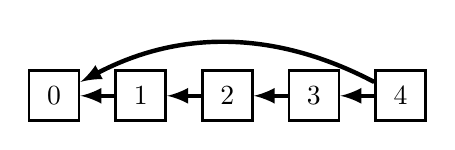
\begin{tikzpicture}[xscale=1.1]
      \foreach \i [count=\x] in {0, 1, 2, 3, 4} {%
        \node[smallsquare] (\i) at (\x, 0) {$\i$};
      }
      \draw[dep] (1) to (0);
      \draw[dep] (2) to (1);
      \draw[dep] (3) to (2);
      \draw[dep, bend right] (4) to (0);
      \draw[dep] (4) to (3);
    \end{tikzpicture}
    \caption{$G_1$}\figlabel{DeadlockBPaxosExampleG1}
  \end{subfigure}
  \hspace{1in}%
  \begin{subfigure}[b]{0.3\textwidth}
    \centering
    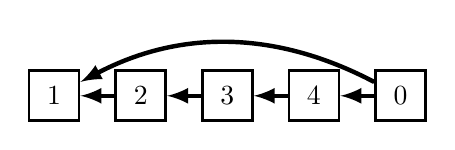
\begin{tikzpicture}[xscale=1.1]
      \foreach \i [count=\x] in {1, 2, 3, 4, 0} {%
        \node[smallsquare] (\i) at (\x, 0) {$\i$};
      }
      \draw[dep, bend right] (0) to (1);
      \draw[dep] (0) to (4);
      \draw[dep] (2) to (1);
      \draw[dep] (3) to (2);
      \draw[dep] (4) to (3);
    \end{tikzpicture}
    \caption{$G_2$}\figlabel{DeadlockBPaxosExampleG2}
  \end{subfigure}

  \vspace{0.2in}

  \begin{subfigure}[b]{0.3\textwidth}
    \centering
    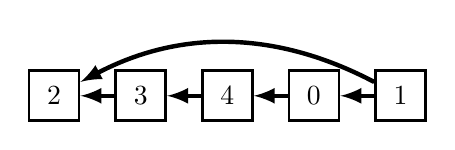
\begin{tikzpicture}[xscale=1.1]
      \foreach \i [count=\x] in {2, 3, 4, 0, 1} {%
        \node[smallsquare] (\i) at (\x, 0) {$\i$};
      }
      \draw[dep] (0) to (4);
      \draw[dep] (1) to (0);
      \draw[dep, bend right] (1) to (2);
      \draw[dep] (3) to (2);
      \draw[dep] (4) to (3);
    \end{tikzpicture}
    \caption{$G_3$}\figlabel{DeadlockBPaxosExampleG3}
  \end{subfigure}
  \hspace{1in}%
  \begin{subfigure}[b]{0.3\textwidth}
    \centering
    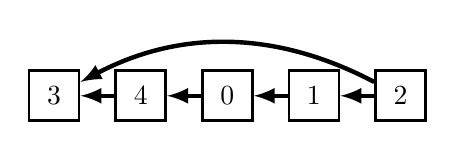
\begin{tikzpicture}[xscale=1.1]
      \foreach \i [count=\x] in {3, 4, 0, 1, 2} {%
        \node[smallsquare] (\i) at (\x, 0) {$\i$};
      }
      \draw[dep] (0) to (4);
      \draw[dep] (1) to (0);
      \draw[dep] (2) to (1);
      \draw[dep, bend right] (2) to (3);
      \draw[dep] (4) to (3);
    \end{tikzpicture}
    \caption{$G_4$}\figlabel{DeadlockBPaxosExampleG4}
  \end{subfigure}

  \vspace{0.2in}

  \begin{subfigure}[b]{0.3\textwidth}
    \centering
    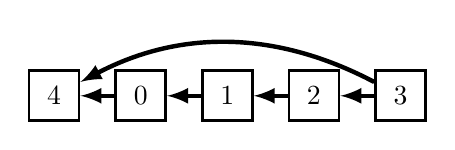
\begin{tikzpicture}[xscale=1.1]
      \foreach \i [count=\x] in {4, 0, 1, 2, 3} {%
        \node[smallsquare] (\i) at (\x, 0) {$\i$};
      }
      \draw[dep] (0) to (4);
      \draw[dep] (1) to (0);
      \draw[dep] (2) to (1);
      \draw[dep] (3) to (2);
      \draw[dep, bend right] (3) to (4);
    \end{tikzpicture}
    \caption{$G_5$}\figlabel{DeadlockBPaxosExampleG5}
  \end{subfigure}

  \caption{A Deadlock BPaxos deadlock}%
  \figlabel{DeadlockBPaxosExample}
\end{figure}
}

Imagine BPaxos node $S$ attempts to recover $I_0$. $\QuorumMajoritySize$
acceptors have voted for $\deps{0} = \set{4}$, but $o_2$ voted for $\set{1,
4}$. Thus, $S$ attempts to recover $I_1$. $\QuorumMajoritySize$ acceptors have
voted for $\deps{1} = \set{0}$, but $o_3$ voted for $\set{0, 2}$, so $S$
attempts to recover $I_2$. This continues until $S$ attempts to recover $I_4$.
$\QuorumMajoritySize$ acceptors have voted for $\deps{4} = \set{3}$, but $o_1$
voted for $\set{0, 3}$, so $S$ attempts to recover $I_0$. This is a deadlock.

Moreover, based on the order in which the $4$ failed nodes processed the five
commands, any four of the five commands could have been chosen. For example, if
the four failed nodes saw the commands in the order $0, 1, 2, 3, 4$, then the
commands $1, 2, 3, 4$ could have been committed on the fast path in round 0.
Or, if the four failed nodes saw the commands in the order $1, 2, 3, 4, 0$,
then the commands $2, 3, 4, 0$ could have been committed on the fast path in
round 0. Because these four nodes have failed, it is impossible for us to know
the order in which they processed the five commands, so it is impossible for us
to know which subset of the commands may have been committed. This shows that
there is no simple fix to \algoref{DeadlockBPaxos} that would allow a Deadlock
BPaxos node to resolve the deadlock.

\TODO[mwhittaker]{%
  There is still one small annoying detail not fully explained in this section.
  It might be possible that in the last else case of \algoref{DeadlockBPaxos},
  a node learns that $R.i$ has already been chosen, but it doesn't know what
  dependencies it has been chosen with. I think that this is actually
  impossible, but I'm not 100\% sure. To be super duper sure that it is
  impossible, we just have to make sure that whenever a node learns that an
  instance has been chosen, it also learns the value that was chosen. This is
  not at all hard to do, but it makes the protocol a little bit more
  cumbersome.
}


In line 1, $b_i$ determines whether there exists some $v \in V$ that satisfies
$O4(v)$. $O4(v)$ is a necessary condition for $v$ to have been chosen in round
$0$, so if no such $v$ exists, then no value could have been chosen in round
$0$. Thus, in line 2, $b_i$ is free to propose any value that maintains
\invref{PrunedDependencies}.
%
Otherwise, there does exist a $v = (x, \deps{I}) \in V$ satisfying $O4(v)$. As
we saw with Unsafe BPaxos, if $v$ was maybe chosen in round $0$, then $b_i$
\emph{must} propose $v$ in order to maintain \invref{ConsensusInvariant}. But
simultaneously to maintain \invref{ConflictInvariant}, $b_i$ must \emph{not}
propose $v$ unless $\deps{I}$ was computed by the dependency service. Unanimous
BPaxos resolved this tension by increasing fast quorum sizes. Deadlock BPaxos
resolves the tension by performing a more sophisticated recovery procedure.  In
particular, $b_i$ does a bit of detective work to conclude either that $v$ was
definitely not chosen in round $0$ (in which case, $b_i$ can propose a
different value) or that $\deps{I}$ happens to be a pruned set of dependencies
(in which case, $b_i$ is safe to propose $v$).

In lines $4$ and $5$, $b_i$ sends $(I, x)$ to the dependency service nodes
co-located with the acceptors in $\Quorum$ and receives the corresponding
dependency service reply $(I, x, \deps{I}_\Quorum)$.%
\footnote{%
  Note that $(I, x)$ messages can be piggybacked on the phase 1a messages
  previously sent by $b_i$. This eliminates the extra round trip.
}
$\deps{I}_\Quorum$ is the union of the dependencies computed by these
co-located dependency service nodes. Moreover, a majority of these co-located
dependency service nodes computed the dependencies of $I$ to be $\deps{I}$
(because $O4(v)$). Thus, $\deps{I} \subseteq \deps{I}_\Quorum$.

Next, $b_i$ enters a for loop in an attempt to prune $\deps{I}_\Quorum$ until
it is equal to $\deps{I}$. That is, $b_i$ attempts to construct a set of
instances $P$ such that $\deps{I} = \deps{I}_\Quorum - P$ is a set of pruned
dependencies. For every, $I' \in \deps{I}_\Quorum - \deps{I}$, $b_i$ first
recovers $I'$ if $b_i$ does not know if a value has been chosen in instance
$I'$. After recovering $I'$, assume $b_i$ learns that $I'$ is chosen with value
$(x', \deps{I'})$. If $x' = \noop$ or if $I \in \deps{I'}$, then $b_i$ can
safely prune $I'$ from $\deps{I}_\Quorum$, so it adds $I'$ to $P$.
%
Otherwise, $b_i$ contacts some quorum $\Quorum'$ of acceptors. If any acceptor
$a_j$ in $\Quorum'$ knows that instance $I$ has already been chosen, then $b_i$
can abort the recovery of $I$ and retrieve the chosen value directly from
$a_j$. Otherwise, in line 19, $b_i$ concludes that $v$ was not chosen in round
$0$ and is free to propose any value that maintains
\invref{PrunedDependencies}. We will explain momentarily why $b_i$ is able to
make such a conclusion. It is not obvious.
%
Finally, if $b_i$ exits the for loop, then it has successfully pruned
$\deps{I}_\Quorum$ into $\deps{I}_\Quorum - P = \deps{I}$ and can safely
propose it without violating \invref{ConsensusInvariant} or
\invref{ConflictInvariant}. As described above, when $b_i$ sends a phase 2a
message with value $v$, it also includes the values chosen in every instance in
$P$.

We now return to line 19 and explain how $b_i$ is able to conclude that $v$ was
not chosen in round $0$. On line 19, $b_i$ has already concluded that $I'$ was
not chosen with $\noop$ and that $I \notin \deps{I'}$. By
\invref{PrunedDependencies}, $\deps{I'} = \deps{I'}_{\mathcal{R}} - P'$ is a
set of pruned dependencies where $\deps{I'}_{\mathcal{R}}$ is a set of
dependencies computed by a quorum $\mathcal{R}$ of dependency service nodes.
Because $I \notin \deps{I'}_{\mathcal{R}} - P'$, either $I \notin
\deps{I'}_{\mathcal{R}}$ or $I \in P'$.
%
$I$ cannot be in $P'$ because if $I'$ were chosen with dependencies
$\deps{I'}_{\mathcal{R}} - P'$, then some quorum of acceptors would have
received $P'$ and learned that $I$ was chosen. But, when $b_i$ contacted the
quorum $\Quorum'$ of acceptors, none knew that $I$ was chosen, and any two
quorums intersect.
%
Thus, $I \notin \deps{I'}_{\mathcal{R}}$. Thus, every dependency service node
in $\mathcal{R}$ processed instance $I'$ before instance $I$. If not, then a
dependency service node in $\mathcal{R}$ would have computed $I$ as a
dependency of $I'$. However, if every dependency service node in $\mathcal{R}$
processed $I'$ before $I$, then there cannot exist a fast quorum of dependency
service nodes that processed $I$ before $I'$. In this case, $v = (x, \deps{I})$
could not have been chosen in round $0$ because it necessitates a fast quorum
of dependency service nodes processing $I$ before $I'$ because $I' \notin
\deps{I}$.

\subsection{Safety}
Deadlock BPaxos maintains \invref{ConsensusInvariant} by implementing Fast
Paxos with the phase 2a tweak outlined in \algoref{FastPaxosTweak} and expanded
in \algoref{DeadlockBPaxos}. As described above, when a node $b_i$ executes
\algoref{DeadlockBPaxos}, it makes sure to propose a value $v$ if $v$ was maybe
chosen in round $0$. $b_i$ proposes a different value in phase 2a only if it
concludes that no value was chosen in round $0$. Thus, \algoref{DeadlockBPaxos}
faithfully implements \algoref{FastPaxosTweak}, and Deadlock BPaxos
successfully maintains \invref{ConsensusInvariant}.
%
As explained above, Deadlock BPaxos maintains \invref{ConflictInvariant} by
maintaining \invref{PrunedDependencies}. The proof that Deadlock BPaxos
maintains \invref{PrunedDependencies} is a straightforward extension of the
proof given in \secref{UnsafeBPaxos} with a case analysis on
\algoref{DeadlockBPaxos} using the arguments presented above.

Unfortunately, while Deadlock BPaxos is safe, it is not very live. There are
certain failure-free situations in which Deadlock BPaxos can permanently
deadlock (see \appendixref{DeadlockExample} for a concrete example). The reason
for this is line 11 of \algoref{DeadlockBPaxos} in which a Deadlock BPaxos node
defers the recovery of one instance for the recovery of another. There exists
executions of Deadlock BPaxos with a chain of instances $I_1, \ldots, I_m$
where the recovery of every instance $I_i$ depends on the recovery of instance
$I_{i+1 \bmod m}$.
